\chapter{Simulator Models}

\section{Basic Components}

\subsection{Inductor}

The presence of an inductor or a capacitor in a circuit introduce dynamic that requires the knowledge of the "past" behavior of the component to represent its quantities at a given time.

An inductor can be described by the following equations: 

\begin{equation}
        v_L(t) = L \frac{di_L(t)}{dt}
\end{equation}

\begin{equation}
        i_L(t) = i_L(t- \Delta t) + \frac{1}{L} \cdot \int_{t- \Delta t}^{t} v_L(\tau) d \tau 
\end{equation}

In dynamic phasors the inductor equations become:

\begin{equation}
        v_L(t) = L \frac{di_L(t)}{dt} + j \omega \cdot L \cdot  i_L(t)
\end{equation}

\begin{equation}
        i_L(t) = i_L(t- \Delta t) +  \int_{t- \Delta t}^{t} \frac{1}{L} \cdot v_L(\tau) -j \omega \cdot i_L(\tau)d \tau 
\end{equation}

A numerical solution for these equations can only be obtained at a finite number of points, therefore a discretization of time is required.
There are different integration methods available to solve the integration problem. The method chosen in this work is the trapezoidal rule.

Given the following equation, that defines the value of a variable $y$ at the point $k+1$.

\begin{equation}
	y(k+1) = y(k) + \int_{t_k}^{t_k+ \Delta t} x(\tau)d \tau
\end{equation}

With the trapezoidal rule $y(k+1)$ is calculated as following:

\begin{equation}
	y(k+1)=y(k)+ \frac{x(k)+x(k+1)}{2} \cdot \Delta t
\end{equation}

Applying trapezoidal rule for the inductor equation:

\begin{equation}
        i_L(k+1) = i_L(k) + \frac{\Delta t}{2} \left[ \frac{1}{L} \cdot v_L(k+1) - j \omega \cdot i_L(k+1) + \frac{1}{L} \cdot v(k) - j \omega \cdot i_L(k) \right]
\end{equation}

Defining:

\begin{align}
	a &= \frac{\Delta t}{2L} \\
	b &= \frac{\Delta t \omega}{2}
\end{align}
		
The equation can be rewritten as

\begin{align}
        i_L(k+1) &= i_L(k) + a \cdot v_L(k+1) - j b \cdot i_L(k+1) + a \cdot v(k) - j b \cdot i_L(k) \\
        i_L(k+1) &= i_L(k) \cdot \frac{1-jb}{1+jb} + \frac{a}{1+jb} \cdot [v_L(k)+v_L(k+1)] \\
        i_L(k+1) &= \frac{1-b^2-j2b}{1+b^2} \cdot i_L(k) + \frac{a-jab}{1+b^2} \left[ v_L(k+1) + v_L(k) \right]
\end{align}

The inductor in calculation step k+1 can be substituted with a resistance $R_L$ in parallel with a current source $I_L(k)$. The value of $I_L(k)$ depends only on the previous time step.

\begin{figure}[ht]
	\centering
	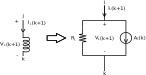
\includegraphics[scale=0.6]{img/Inductor.png} 
	\caption{Equivalent circuit of an Inductor}
	\label{fig:Inductor}
\end{figure}


\begin{equation}
	I_L(k) = i_L(k) \cdot \frac{1-b^2-2bj}{1+b^2} + v_L(k) \cdot \frac{a-jab}{1+b^2}
\end{equation}

\begin{equation}
	R_L = \frac{1+b^2}{a-jab}
\end{equation}	


\subsection{Capacitor}

The same approach used for the inductor is used now for the capacitor.
A capacitor can be described by the following equations:

\begin{equation}
	i_C(t)= C \frac{d v_c}{dt}
\end{equation}

\begin{equation}
	v_C(t)= v_C(t - \Delta t) + \frac{1}{C} \int_{t - \Delta t}^{t} i_C (\tau) d \tau
\end{equation}

In dynamic phasor the capacitor equations become:

\begin{equation}
        i_C(t)= C \frac{d v_c}{dt} + j \omega \cdot C \cdot v_C(t)
\end{equation}

\begin{equation}
        v_C(t) = v_C(t- \Delta t) +  \int_{t- \Delta t}^{t} \frac{1}{C} \cdot i_C(\tau) -j \omega \cdot v_C(\tau)d \tau 
\end{equation}

Applying trapezoidal rule for the capacitor equation:

\begin{equation}
        v_C(k+1) = v_C(k) + \frac{\Delta t}{2} \left[ \frac{1}{C} \cdot i_C(k+1) - j \omega \cdot v_C(k+1) + \frac{1}{C} \cdot i_C(k) - j \omega \cdot v_C(k) \right]
\end{equation}

Defining:
\begin{align}
        a &= \frac{\Delta t}{2C} \\
        b &= \frac{\Delta t \omega}{2}
\end{align}

\begin{align}
        v_C(k+1) &= v_C(k) + a \cdot i_C(k+1) - j b \cdot v_C(k+1) + a \cdot i_C(k) - j b \cdot v_C(k) \\
        i_C(k+1) &= -i_C(k) + \frac{1+jb}{a} \cdot v_C(k+1) - \frac{1-jb}{a} \cdot v_C(k)
\end{align}

The capacitor in calculation step k+1 can also be substituted with a resistance $R_C$ in parallel with a current source $I_C(k)$. The value of $I_C(k)$ depends only on the previous time step.

\begin{figure}[ht]
	\centering
	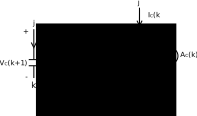
\includegraphics[scale=0.6]{img/Capacitor.png} 
	\caption{Equivalent circuit of a Capacitor}
	\label{fig:Capacitor}
\end{figure}

\begin{equation}
	R_C = \frac{a}{1+jb}
\end{equation}

\begin{equation}
	I_C = \frac{1-jb}{a} v_C(k) + i_C(k)
\end{equation}

\subsection{Voltage Source}

A real voltage source can be represented as a voltage source $V$ in series with a resistance $R$, with

\begin{equation}
V=Va \cdot cos(\omega t + \phi)
\end{equation}
In dynamic phasors the voltage source V becomes

\begin{equation}
V = Va \cdot cos (\phi) + jVa \cdot sin(\phi) 
\end{equation}

As nodal analysis does not support voltage source, it is transformed to a current source using the Norton Equivalent as shown in figure \ref{fig:Real_Voltage_Source}.

\begin{figure}[ht]
	\centering
	\includegraphics[scale=0.5]{img/VoltageSourceRes.png} 
	\caption{Real Voltage Source}
	\label{fig:Real_Voltage_Source}
\end{figure}

\subsection{Ideal Voltage Source}
An ideal voltage source does not have the resistance in series and therefore cannot be transformed to a current source. In this case, the modified nodal analysis approach is used. The voltage source is represented, by adding a new equation to the problem and adding the current trough the voltage source as unknown. 

\begin{figure}
	\centering
	\includegraphics[scale=0.6]{img/IdealVoltageSource.png}
	\caption{Matrix stamp of ideal voltage source}
	\label{fig:Ideal_Voltage_Source}
\end{figure}

For a voltage source between node j and node k. The added equation is the following:
\begin{equation}
e_j - e_k = V
\end{equation}
Moreover, the current trough the voltage source is added in the equation of node j and subtracted in the equation of node k.





\section{Synchronous Machine}

The model is according to \cite{wang2010methods} and \cite{kundur1994power}. 

\subsubsection{Prerequisites}
Park's transformation is commonly used to achieve a model with static parameters:
%
\begin{equation}
\mathbf{K_s} = \frac{2}{3}
 \begin{bmatrix} 
  \cos \theta & \cos(\theta-\frac{2\pi}{3}) & \cos(\theta+\frac{2\pi}{3}) \\
  \sin \theta & \sin(\theta-\frac{2\pi}{3}) & \sin(\theta+\frac{2\pi}{3}) \\
  \frac{1}{2} & \frac{1}{2} & \frac{1}{2}
 \end{bmatrix}
\end{equation}
%
Note that the scaling factor $\frac{2}{3}$, which ensures an equal length of the current dq-axis and stator reference frame current, is not always used. 
%
\begin{equation}
(\mathbf{K_s})^{-1} = 
 \begin{bmatrix} 
  \cos \theta & \sin \theta & 1 \\
  \cos(\theta-\frac{2\pi}{3}) & \sin(\theta-\frac{2\pi}{3}) & 1 \\
  \cos(\theta+\frac{2\pi}{3}) & \sin(\theta+\frac{2\pi}{3}) & 1
 \end{bmatrix}
\end{equation}
%
where $\theta$ is the rotor angle in this case.

\subsubsection{Model}

The mechanical equations are:
%
\begin{align}
\frac{d\theta_r}{dt} &= \omega_r \label{eq:d_theta} \\
\frac{d\omega_r}{dt} &= \frac{P}{2J} (T_e-T_m) \label{eq:d_omega}
\end{align}
%
where $\theta_r$ is the rotor position, $\omega_r$ is the angular electrical speed, $P$ is the number of poles, $J$ is the moment of inertia, $T_m$ and $T_e$ are the mechanical and electrical torque, respectively. Motor convention is used for all models. 

The electrical model in the phase domain is described by the following equations:
%
\begin{align}
  \mathbf{v}_{abcs} &= \mathbf{R}_s \mathbf{i}_{abcs} + \frac{d}{dt} \boldsymbol{\lambda}_{abcs} \\
  \mathbf{v}_{qdr} &= \mathbf{R}_r \mathbf{i}_{qdr} + \frac{d}{dt}  \boldsymbol{\lambda}_{qdr}
\end{align}
%
where
%
\begin{align}
  \mathbf{v}_{abcs} &= 
  \begin{pmatrix}
    v_{as} & v_{bs} & v_{cs}
  \end{pmatrix}^T \\
  %  
  \mathbf{v}_{qdr} &= 
  \begin{pmatrix}
    v_{kq1} & v_{kq2} & v_{fd} & v_{kd} 
  \end{pmatrix}^T \\
  %
  \mathbf{i}_{abcs} &= 
  \begin{pmatrix}
    i_{as} & i_{bs} & i_{cs}
  \end{pmatrix}^T \\
  %  
  \mathbf{i}_{qdr} &= 
  \begin{pmatrix}
    i_{kq1} & i_{kq2} & i_{fd} & i_{kd} 
  \end{pmatrix}^T \\
  %
  \boldsymbol{\lambda}_{abcs} &= 
  \begin{pmatrix}
    \lambda_{as} & \lambda_{bs} & \lambda_{cs}
  \end{pmatrix}^T \\
  %  
  \boldsymbol{\lambda}_{qdr} &= 
  \begin{pmatrix}
    \lambda_{kq1} & \lambda_{kq2} & \lambda_{fd} & \lambda_{kd} 
  \end{pmatrix}^T \\
  %
  \mathbf{R}_s &= diag
  \begin{bmatrix}
    r_s & r_s & r_s 
  \end{bmatrix} \\
  %
  \mathbf{R}_r &= diag
  \begin{bmatrix}
    r_{kq1} & r_{kq2} & r_{fd} & r_{kd}
  \end{bmatrix}
\end{align}
%
The flux linkages are:
%
\begin{align}
  \boldsymbol{\lambda}_{abcs} &= \mathbf{L}_{ss} \mathbf{i}_{abcs} + \mathbf{L}_{sr} \mathbf{i}_{qdr}  \\
  \boldsymbol{\lambda}_{qdr} &= \mathbf{L}_{rs} \mathbf{i}_{abcs} + \mathbf{L}_{rr} \mathbf{i}_{qdr}
\end{align}
%
where the inductances are time variant variables as defined in \cite{krause2002sudhoff}.
TODO: electromagnetic torque

\subsubsection{Equations in Rotor Reference Frame}

This section depicts the synchronous generator equations in terms of machine variables referred to the stator windings which is indicated by the prime symbol. Due to the transform of the stator variables to the rotor reference frame, the stator equations change, whereas the rotor equations remain the same.
%
\begin{equation}
  \begin{pmatrix}
    \mathbf{v}_{qd0s} \\
    \mathbf{v}_{qdr}
  \end{pmatrix}
  =  
  \mathbf{R}'
  \begin{pmatrix}
    \mathbf{i}_{qd0s} \\
    \mathbf{i}_{qdr}'
  \end{pmatrix}
  +
  \frac{d}{dt}
  \begin{pmatrix}
    \boldsymbol{\lambda}_{qd0s} \\
    \boldsymbol{\lambda}_{qdr}'
  \end{pmatrix}
  + \omega_r
  \begin{pmatrix}
    \boldsymbol{\lambda}_{dqs} \\
    0
  \end{pmatrix}
\end{equation}
%
where
%
\begin{align}
  \mathbf{R}' &= diag
  \begin{bmatrix}
    r_s & r_s & r_s & r_{kq1}' & r_{kq2}' & r_{fd}' & r_{kd}' 
  \end{bmatrix} \\
  \boldsymbol{\lambda}_{dqs} &= 
  \begin{pmatrix}
    \lambda_{ds} & -\lambda_{qs} & 0
  \end{pmatrix}^T
\end{align}
%
The flux linkages are:
%
\begin{equation}
  \begin{pmatrix}
    \boldsymbol{\lambda}_{qd0s} \\
    \boldsymbol{\lambda}_{qdr}'
  \end{pmatrix}
  =
  \begin{bmatrix}
    \mathbf{L}_{qdss} & \mathbf{L}_{qdsr}' \\
    \mathbf{L}_{qdrs}' & \mathbf{L}_{rr}'    
  \end{bmatrix}
  \begin{pmatrix}
    \mathbf{i}_{qd0s} \\
    \mathbf{i}_{qdr}'
  \end{pmatrix}
  \label{eq:flux}
\end{equation}
%
where
%
\begin{align}
  \mathbf{L}_{qdss} &= 
  \begin{bmatrix}
    L_{q} & 0 & 0 \\
    0 & L_{d} & 0 \\
    0 & 0 & L_{ls}
  \end{bmatrix} \\
  %  
  \mathbf{L}_{qdsr}' &= 
  \begin{bmatrix}
    L_{mq} & L_{mq} & 0 & 0 \\
    0 & 0 & L_{md} & L_{md} \\
    0 & 0 & 0 & 0
  \end{bmatrix} \\
  %
  \mathbf{L}_{qdrs}' &=
  \begin{bmatrix}
    L_{mq} & 0 & 0 \\
    L_{mq} & 0 & 0 \\
    0 & L_{md} & 0 \\
    0 & L_{md} & 0
  \end{bmatrix} \\
  %
  \mathbf{L}_{rr}' &=
  \begin{bmatrix}
    L_{kq1}' & L_{mq} & 0 & 0 \\
    L_{mq} & L_{kq2}' & 0 & 0 \\
    0 & 0 & L_{fd}' & L_{md} \\
    0 & 0 & L_{md} & L_{kd}'
  \end{bmatrix} \\
  %
\end{align}
%
with 
%
\begin{align}
  L_{q} &= L_{ls} + L_{mq} \\
  L_{d} &= L_{ls} + L_{md} \\
  L_{kq1'} &= L_{lkq1'} + L_{mq} \\
  L_{kq2'} &= L_{lkq2'} + L_{mq} \\
  L_{fd'} &= L_{lfd'} + L_{md} \\
  L_{kd'} &= L_{lkd'} + L_{md}
\end{align}

\subsubsection{State Space Model}
The flux linkage variables are chosen as electrical states of the state-space representation. Then, the currents can be calculated from equation \ref{eq:flux}.
%
\begin{equation}
  \frac{d}{dt}
  \begin{pmatrix}
    \boldsymbol{\lambda}_{qd0s} \\
    \boldsymbol{\lambda}_{qdr}'
  \end{pmatrix}
  =
  \begin{pmatrix}
    \mathbf{v}_{qd0s} \\
    \mathbf{v}_{qdr}'
  \end{pmatrix}
  - \mathbf{R}'
  \begin{pmatrix}
    \mathbf{i}_{qd0s} \\
    \mathbf{i}_{qdr}'
  \end{pmatrix}
  - \omega_r
  \begin{pmatrix}
    \boldsymbol{\lambda}_{dqs} \\
    0
  \end{pmatrix}
\end{equation}
%
or
%
\begin{equation}
  \frac{d}{dt}
  \begin{pmatrix}
    \boldsymbol{\lambda}_{qd0s} \\
    \boldsymbol{\lambda}_{qdr}'
  \end{pmatrix}
  =
  \begin{pmatrix}
    \mathbf{v}_{qd0s} \\
    \mathbf{v}_{qdr}'
  \end{pmatrix}
  - \mathbf{R}'
  \begin{bmatrix}
    \mathbf{L}_{qdss} & \mathbf{L}_{qdsr}' \\
    \mathbf{L}_{qdrs}' & \mathbf{L}_{rr}'    
  \end{bmatrix}^{-1}
  \begin{pmatrix}
    \boldsymbol{\lambda}_{qd0s} \\
    \boldsymbol{\lambda}_{qdr}
  \end{pmatrix}  
    - \omega_r
  \begin{pmatrix}
    \boldsymbol{\lambda}_{dqs} \\
    0
  \end{pmatrix}
\end{equation}
%
since the currents are 
%
\begin{align} 
   \begin{pmatrix}
    \mathbf{i}_{qd0s} \\
    \mathbf{i}_{qdr}'
  \end{pmatrix}
  = 
  \begin{bmatrix}
    \mathbf{L}_{qdss} & \mathbf{L}_{qdsr}' \\
    \mathbf{L}_{qdrs}' & \mathbf{L}_{rr}'    
  \end{bmatrix}^{-1}
  \begin{pmatrix}
    \boldsymbol{\lambda}_{qd0s} \\
    \boldsymbol{\lambda}_{qdr}
  \end{pmatrix}
\end{align}
%
The voltages of the damper windings are always zero since they are short-circuited. The state-space representation of the mechanical part is
%
\begin{align}
 \frac{d}{dt}
  \begin{pmatrix}
    \theta_r \\
    \omega_r
  \end{pmatrix}
  =
  \begin{bmatrix}
    0 & 1 \\
    0 & 0 \\
  \end{bmatrix}
  \begin{pmatrix}
    \theta_r \\
    \omega_r
  \end{pmatrix}
  + 
  \begin{pmatrix}
    0 \\
    \frac{P}{2J} \left( T_e - T_m \right)
  \end{pmatrix} 
\end{align}
%
where the electric torque is
%
\begin{equation}
  T_e = \frac{3P}{4} \left( \boldsymbol{\lambda}_{ds} \mathbf{i}_{qs} - \boldsymbol{\lambda}_{qs} \mathbf{i}_{ds} \right)
\end{equation}
%

\subsubsection{Alternative State Space Representation}
Defining q- and d-axis flux linkages 
%
\begin{align}
  \lambda_{mq} &= L_{mq} \left( i_{qs} + i_{kq1}' + i_{kq2}' \right) \\
  \lambda_{md} &= L_{md} \left( i_{ds} + i_{fd}' + i_{kd}' \right) \\
\end{align}
%
allows to rewrite the equations